\section{Implementation}
\label{sec:approach-impl}
\subsection{System architecture}
- Diagram of the system architecture 
(Client-side, server-side + database side and communication with each side).

\begin{figure}[h]
	\begin{center}
		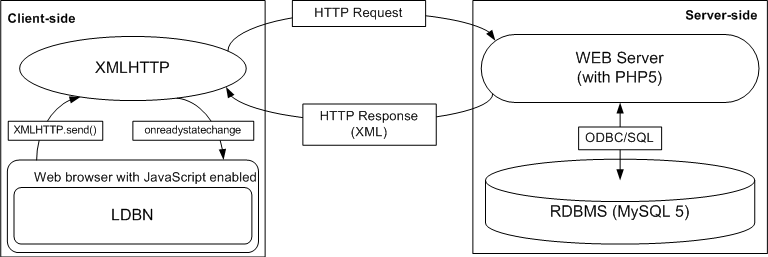
\includegraphics[width=0.9\textwidth]{./img/design01.png}
		\caption{LDBN - System Architecture}
		\label{fig:sysarch}
	\end{center}
\end{figure}

- Function distribution (+ diagram) -> decentralized architecture -> less 
server load.

\begin{figure}[h]
	\begin{center}
		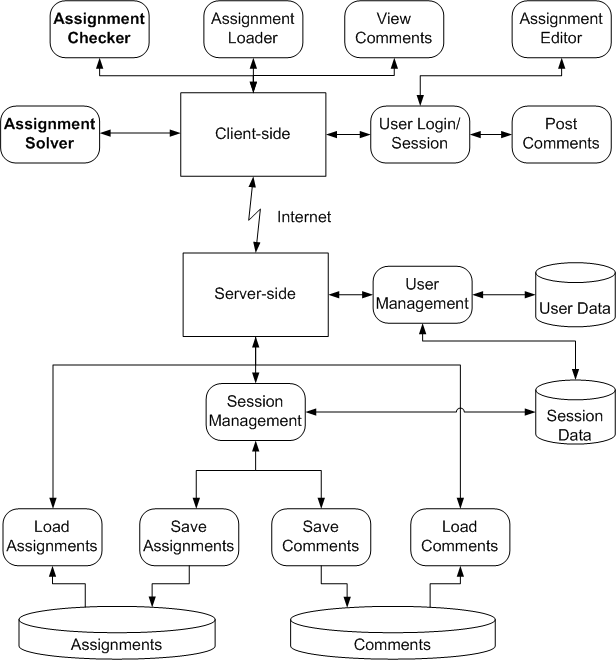
\includegraphics[width=0.85\textwidth]{./img/functions01.png}
		\caption{LDBN - Functions Destribution}
		\label{fig:funcdist}
	\end{center}
\end{figure}

\subsection{Client-side}

\begin{figure}[h]
	\begin{center}
		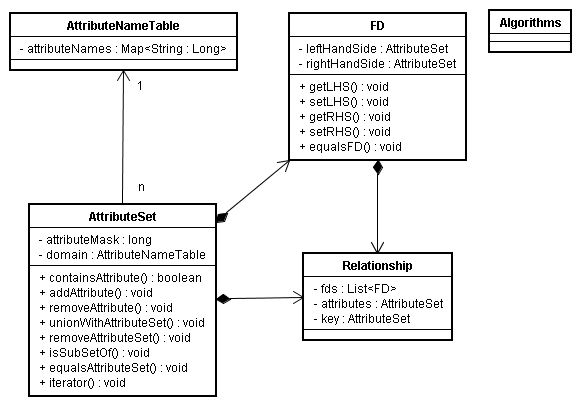
\includegraphics[width=0.8\textwidth]{./img/uml01.png}
		\caption{LDBN - Core Classes}
		\label{fig:coreuml}
	\end{center}
\end{figure}

- Algorithms and data structures + (UML)

-- algorithms and caching results.

-- efficient data structure with bitwise operations (32 bits).

-- Why not to use long (64 bits) variables in a JavaScript environment.

- User interface

-- Easy and fast to use interface -> benefits

-- Drag and Drop and traditional approach of inputing data.

-- Solving Assignments.

-- Creating Assignments.

- Interaction with the server

-- Saving, loading assignments.

-- Exporting and importing -> benefits (limitations of JavaScript - could not set/read headers, thus require the use of PHP).
 
-- User management.

-- Posting comments -> benefits.

\subsection{Server-side}
- brief introduction to PHP and MySQL interaction and to the responses to the client side.

- Handling errors and warning with PHP and sending them back to the client -> use of the "die" command with a proper XML response.


\section{Security issues}
- Validating user input.

- Code injections.

- SQL injections.

- Password management.

- others...